%!TEX root = ../Report.tex
%************************************************

% Detail design

\chapter{Introduction}
In this part the design of the application the end user will use will be discussed in detail. Topics covered include the final selection of algorithms in the application. The design of the user interface. A high level overview of the data structures used. The functionality and features of the application and finally some additional considerations will be reviewed.

\chapter{Technology, Platform and Programming Language}
Some algorithms and features lend themselves to being implemented more easily in certain languages than other. Some implementations of the algorithms considered are notoriously difficult and external libraries were used in this. Thus a programming language needs to be chosen that does not constrain the functionality of the application. 
The three languages with most support include:
\begin{enumerate}
\item Python
\item C\# (and other .NET languages)
\item Java
\item C++
\end{enumerate}
Ranked according to subjective estimates on the amount of programming time required, with C++ taking the most time.

Machine learning libraries exist for all of the above mentioned languages. Python has poor support for rich user interfaces. Java is a good contender and is cross platform. Thus in order to make a final selection the consideration is made to the end user.  .NET languages fascillate the \ac{WPF} - a graphical system for rendering user interfaces, which will allow a rich user experience to be developed.
\\
\\
Winner: \emph{C\#}\footnote{The algorithmic code is cross platform and can be run through Mono, even though the graphical front end developed in \ac{WPF} cannot.}

This additionally has the following advantages:
\begin{enumerate}
\item Ability to easily create rich user interfaces.
\item C\# runs on the CLR and allows access to the large .NET library\footnote{Additionally the IKVM project allows access to Java libraries}
\item Powerful language constructs such as operator overloading, event handling, delegates, powerful multithreading support and generics.
\end{enumerate}


\chapter{Selection of algorithms}
In this chapter the selected algorithms for the end user application are chosen.
The algorithms for consideration are:
\begin{enumerate}
\item Melody generation with Genetic Algorithms
\item Melody generation with Hidden Markov Models
\item Accompaniment geneartion with Hidden Markov Models
\item Accompaniment generation with a \ac{LSTM} network
\item Accompaniment genereation with a feed forward \ac{ANN}
\item Instrumental generation with Markov Chains
\end{enumerate}

The selection of algorithms will be done by means of elimination. Algorithms that yielded sub minumum results will not be selected for inclusion into the end user application.

\chapter{Features and Functionality}
The main goal of the application is to generate melodies according to a certain styles. The user is to selection a certain category of music and the application will generate a musical piece in that style. The premise is to generate the melodies in a certain style using machine learning techniques that will use the data present in the corpus of MIDI files. 

Since training machine learning algorithms take up a lot of time it is not feasible to train the algorithm on the fly. Training will take place beforehand and the resulting data structure of the algorithm will be cached to a file. 
For example a Neural Network will save its topology and weights to a file; this allows the application to load the file, present inputs to the neural network and output a result without spending time learning the optimal weights for the network.

Additional features would be to allow the user to save a generated melody to a file (in \ac{MIDI} or a custom file format), load or play an existing \ac{MIDI} file (for comparison or other aims), re-randomize a generated composition and view more information or properties of the generated music piece.

The application is to be used by end users which do not have background on machine learning. The application is be as user as friendly as possible while still having flexibility in composing songs. The user interface is to visually display the song and playback of it. Playback functionality such as playing and stopping a song are mandatory.

To summarize, the application will:
\begin{enumerate}
\item Implement the selected algorithms and allow them to be used for song generation.
\item Allow saving and loading of \ac{MIDI} files
\item Generate a monophonic melody according to a certain style. Allow the user to select which algorithm to use and adjust high level parameters
\item Playback functionality including playing, pausing and stop a song. 
\item Feature a user friendly interface.
\item Visually display the generated melody.
\item Allow the user to randomize the song based on the selected settings.
\item Cache machine learning data to improve performance of the application
\end{enumerate}

\chapter{Graphical user interface}
In this chapter the design of the graphical user interface is presented, along with the features and functionality of the application.

As mentioned above the user interface is to have the following features
\begin{itemize}
\item Visually display the generated song
\item Selecting the category of melodies to be generated
\item Select algorithm and high level parameters
\item Buttons to allow for saving, loading, pausing, pausing, stopping and playing of songs
\end{itemize}

The user interface will be developed using \ac{WPF} and \ac{XAML}.

\begin{figure}
\centerline{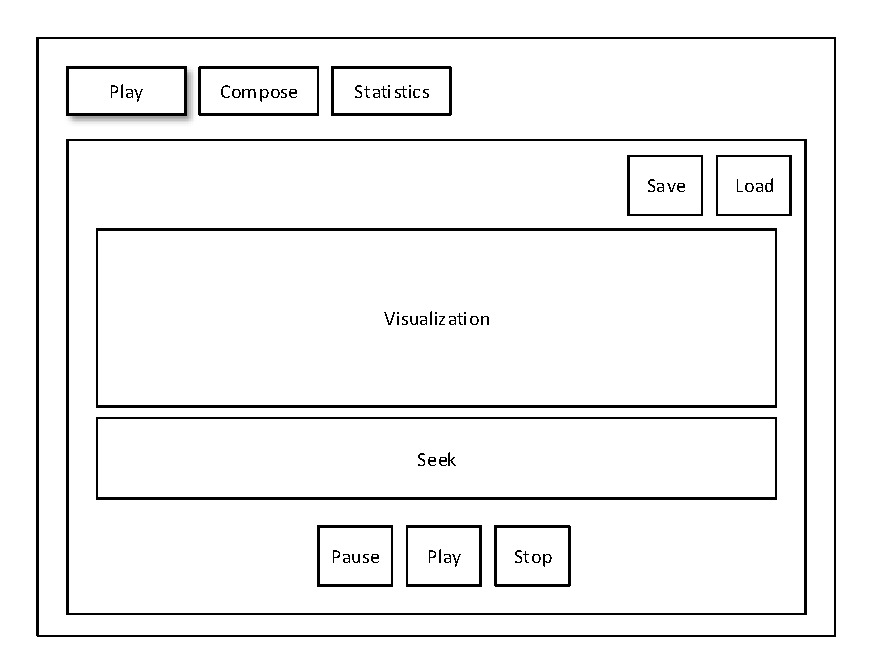
\includegraphics[width=400px]{../images/ui_play.pdf}}
\caption{User interface for playback functionality}
\label{ims:uiplay}
\end{figure}

\begin{figure}
\centerline{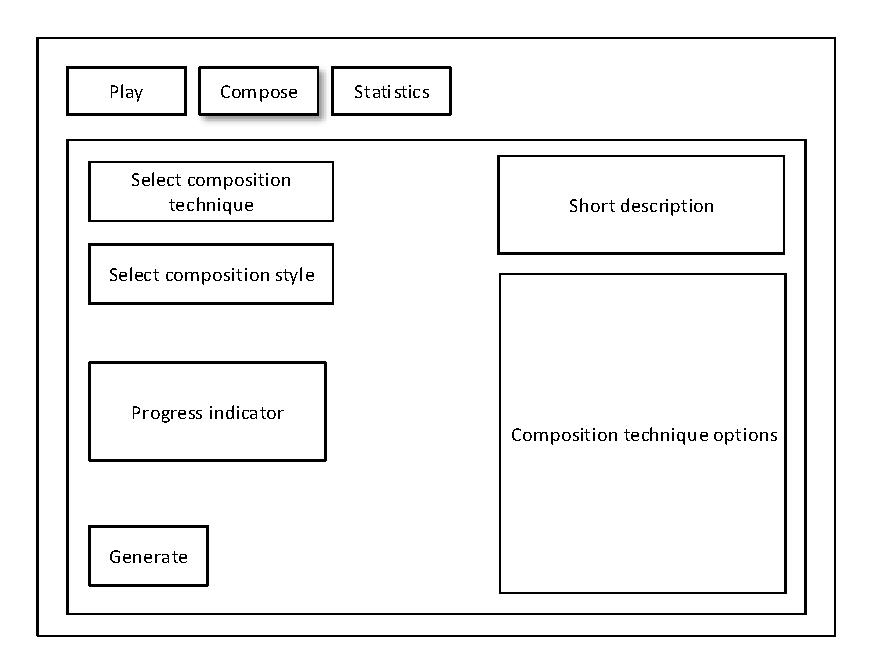
\includegraphics[width=400px]{../images/ui_compose.pdf}}
\caption{User interface for composition functionality}
\label{ims:uicompose}
\end{figure}

\begin{figure}
\centerline{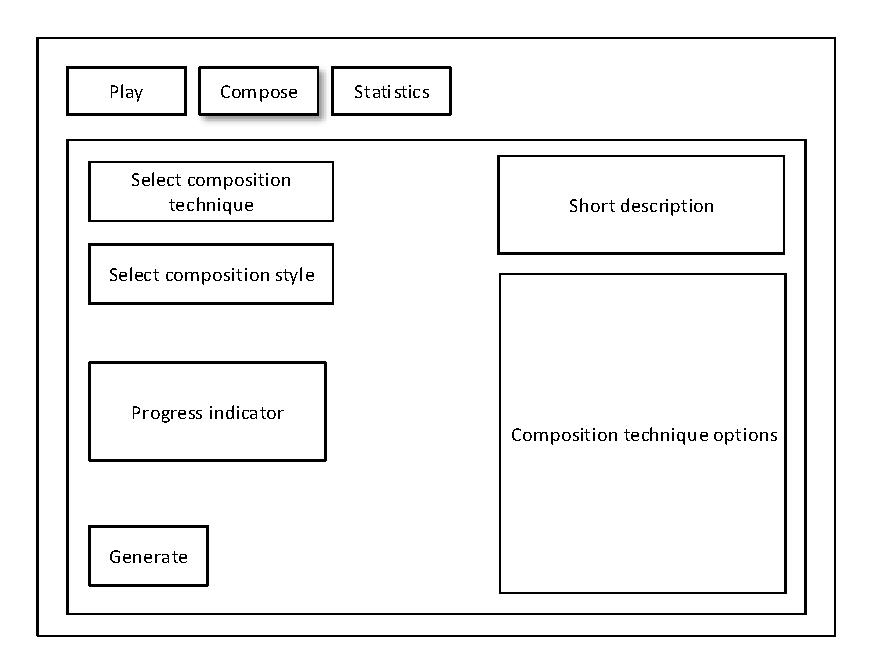
\includegraphics[width=400px]{../images/ui_melody.pdf}}
\caption{User interface for melody generation}
\label{ims:uicompose}
\end{figure}

\begin{figure}
\centerline{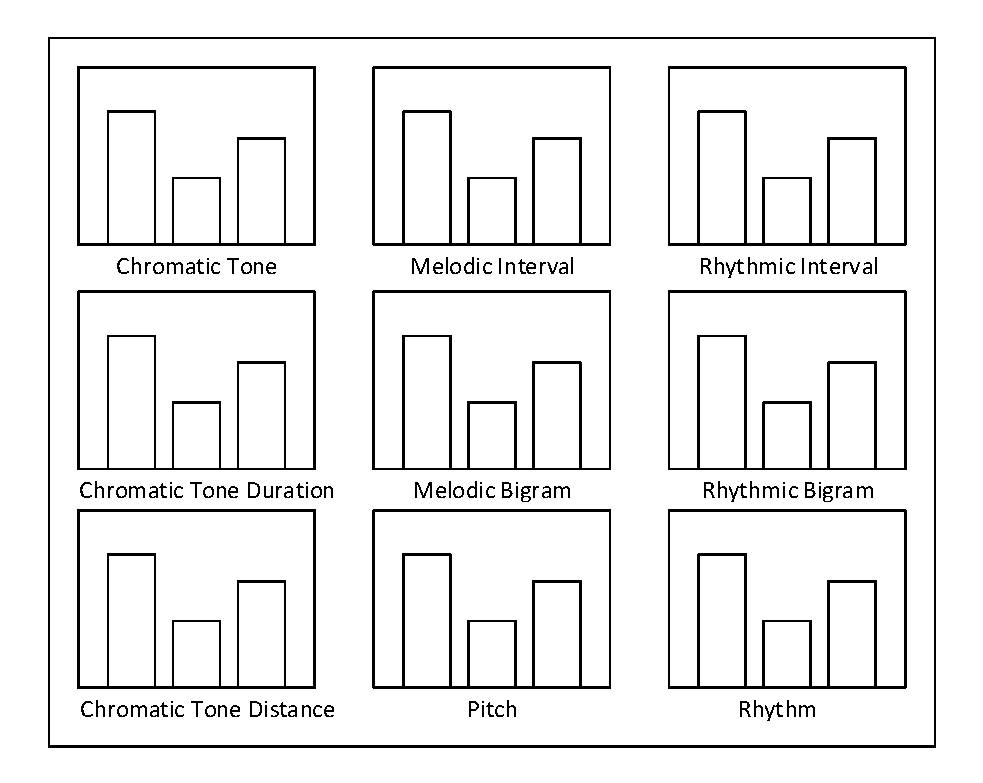
\includegraphics[width=400px]{../images/ui_metrics.pdf}}
\caption{User interface for displaying metrics of a melody}
\label{ims:uimetrics}
\end{figure}




% Functionality and features
% Design
\chapter{Final considerations}